% ============================================================
% Praktická část, bod 5: Testování, nasazení aplikace do provozu
% a vyhodnocení zpětné vazby od zaměstnanců
% Oddíly označené [DOPLNIT] dopíše autor.
% ============================================================
\chapter{Testování, nasazení aplikace do provozu a~vyhodnocení zpětné vazby od zaměstnanců}\label{kap:testovani}

\section{Přístup k~testování}\label{sec:testovani-pristup}

Sommerville rozlišuje dvě otázky, na které testování odpovídá. \emph{Verifikace} ověřuje, zda software splňuje stanovené funkční a~nefunkční požadavky. \emph{Validace} ověřuje, zda software dělá to, co zákazník skutečně očekává \cite[s.~228]{Sommerville2016}. Komerční software podle něj prochází třemi fázemi testování: \emph{vývojovým testováním} během vývoje, \emph{testováním vydání}, kdy se ověřuje celá verze před předáním uživatelům, a~\emph{uživatelským testováním} v~prostředí uživatele \cite[s.~231]{Sommerville2016}.

Vývojové testování se dále dělí na testování jednotek (jednotlivých funkcí a~tříd), testování komponent a~testování systému jako celku \cite[s.~232]{Sommerville2016}. Automatizované testy jsou zapsány jako program, který se spustí při každé změně. Jsou rychlejší než ruční testování, zejména u~\emph{regresního testování}, kdy se po změně znovu spustí všechny dřívější testy a~ověří se, že změna nic nerozbila \cite[s.~231]{Sommerville2016}. Automaticky však nelze otestovat, jak rozhraní vypadá, proto se automatické testy doplňují ručním testováním \cite[s.~231]{Sommerville2016}.

Aplikace byla testována ve všech třech fázích. Vývojové testování tvoří automatické testy a~ruční zkoušky v~prohlížeči, testováním vydání je ověření celé verze na čisté instalaci a~uživatelským testováním je pilotní provoz ve firmě (oddíl~\ref{sec:nasazeni}).

\section{Testovací prostředí}\label{sec:testovani-prostredi}

Aplikace byla testována na vývojovém počítači autora. % [DOPLNIT] ověřit a doplnit údaje
\begin{itemize}
\item počítač: Lenovo Legion~7, operační systém Windows~11 Home 24H2, procesor Intel Core i9 14900HX , paměť RAM 32GB,
\item Python~3.13 a~Django~5.2,
\item databáze SQLite (vývojová instalace) a~PostgreSQL (instalace v~Dockeru, která odpovídá provozu ve firmě),
\item webový prohlížeč Mozilla FireFox.
\end{itemize}

Aplikace se vyvíjí a~průběžně testuje nad databází SQLite. Ta je uložena v~jednom souboru a~nevyžaduje instalaci databázového serveru, takže vývoj a~spouštění testů jsou jednoduché a~rychlé. Ve firmě však aplikace poběží nad databází PostgreSQL v~Dockeru, která lépe zvládá souběžnou práci více uživatelů. Oba systémy se v~některých podrobnostech liší, například v~kontrole integritních omezení nebo v~porovnávání textu. Aplikace k~databázi přistupuje jen přes ORM frameworku Django (oddíl~\ref{sec:principy-orm}), takže stejný kód funguje nad oběma systémy. Aby se ověřilo, že se aplikace chová stejně i~v~reálném provozu, byly všechny automatické testy spuštěny nad SQLite i~nad PostgreSQL.

\section{Automatické testy}\label{sec:testovani-automaticke}

Automatické testy jsou napsány pomocí testovacího nástroje frameworku Django a~jsou uloženy v~souboru \path{core/tests.py}. Spouští se příkazem \texttt{python manage.py test core}. Každý test si vytvoří vlastní prázdnou databázi, takže výsledek nezávisí na datech uložených v~aplikaci. Testy pokrývají části aplikace, ve kterých by chyba měla největší následky: správnost dokladů, integritu dat, oprávnění a~bezpečnost. Přehled všech testů s~popisem toho, co ověřují, a~výsledky jejich spuštění nad databázemi SQLite a~PostgreSQL jsou v~dokumentaci aplikace\footnote{\url{https://github.com/MajkyyQ/BusinessManager/blob/main/docs/09-vyvoj-a-testovani.md}}.

\subsection{Testy bezpečnosti}

Zvláštní pozornost byla věnována útoku SQL injection, který popisuje oddíl~\ref{sec:principy-sql-injection}. Testy zkoušejí přihlášení s~devíti typickými útočnými řetězci ve jménu, v~hesle i~v~obou polích zároveň a~ověřují, že se žádný pokus nepřihlásí a~tabulka uživatelů zůstane beze změny. Dále ověřují, že útočné řetězce ve vyhledávání a~v~parametru řazení seznamu nevrátí cizí data ani nezpůsobí chybu. Podrobnosti jsou v~oddílu~\ref{sec:db-sql-injection}.

\subsection{Bezpečnostní audit}\label{sec:bezpecnostni-audit}

Před zveřejněním aplikace jako open source prošel zdrojový kód aplikace i~modulu Odesílání e-mailů bezpečnostním auditem. Audit postupoval podle metodiky \emph{security-audit}, která za chybu považuje jen porušení skutečné hranice důvěry. U~každého nálezu proto musí být jasné, kdo chybu může zneužít, co tím získá a~která kontrola v~aplikaci selhala. Obecná doporučení bez konkrétního dopadu se vedou zvlášť jako doporučení pro provoz.

Audit vycházel z~toho, pro jaký provoz je aplikace navržená. Aplikace je navržená pro malou firmu v~uzavřené firemní síti. Chrání data před uživateli bez oprávnění a~před lidmi v~síti bez účtu. Nechrání před tím, kdo má přístup přímo k~serverovému PC, protože to patří k~zabezpečení počítače, ne aplikace. Kdo má přístup k~serverovému počítači fyzicky nebo jako jeho správce, má přístup i~k~databázi a~souborům a~žádné zabezpečení uvnitř aplikace ho nezastaví. Útočník ve stejné síti ale k~databázi přístup nemá, protože se databáze do sítě nepublikuje, a~bez účtu uvidí jen přihlašovací stránku. Aplikace také není určená k~vystavení do internetu.

Audit dále vycházel z~rolí a~oprávnění aplikace a~z~toho, odkud do aplikace přicházejí data. Posuzovaly se tyto hranice důvěry:
\begin{itemize}
	\item nepřihlášený návštěvník ve firemní síti nesmí vidět žádnou stránku ani soubor kromě přihlášení a~průvodce prvním spuštěním,
	\item zaměstnanec se základní rolí nesmí vidět doklady bez oprávnění, měnit nastavení, mazat cizí záznamy ani získat vyšší oprávnění,
	\item technik a~administrativa nesmí překročit oprávnění své role,
	\item uživatel s~oprávněním Nastavení nesmí převzít účet hlavního administrátora,
	\item soubor od zákazníka nebo dodavatele (fotka, objednávka, faktura ISDOC) nesmí po nahrání ohrozit aplikaci ani její uživatele.
\end{itemize}

Audit našel šest chyb, žádná z~nich nebyla zneužitelná bez přihlášení. Nejzávažnější umožňovala zaměstnanci se základní rolí nahrát jako přílohu soubor se skriptem, který by se po otevření administrátorem spustil s~jeho právy. Všechny chyby byly opraveny a~každou opravu ověřuje automatický test. Prověřené oblasti kódu, jednotlivé nálezy, jejich opravy a~testy podrobně popisuje dokumentace aplikace.

Z~doporučení auditu byla s~ohledem na popsaný provoz zapracována jen základní opatření. Aplikace se bez konfiguračního souboru nespouští v~ladicím režimu ani s~tajným klíčem známým z~veřejného repozitáře, což je důležité hlavně pro zveřejnění jako open source. Velikost nahrávaných souborů je omezená na 50~MB pro jeden soubor a~500~MB pro jedno nahrání, aby jeden uživatel nemohl zaplnit disk serverového počítače; limit stačí na běžné fotky z~telefonu i~naskenované dokumenty. Heslo k~e-mailové schránce, které aplikace potřebuje při každém odeslání a~nemůže ho proto uložit jen jako otisk jako hesla k~účtům, se ukládá zašifrované klíčem z~konfiguračního souboru, takže ho nelze přečíst z~databáze ani z~její zálohy. Skript pro zálohování nově kopíruje poslední zálohu na jiný disk nebo počítač (oddíl~\ref{sec:zalohovani}). Složitější ochrany, jako omezení počtu pokusů o~přihlášení nebo provoz přes HTTPS, zůstávají doporučením pro případ, že by se aplikace používala v~otevřenější síti. Přístup zvenku, například z~telefonu na výjezdu, je vhodné řešit soukromou sítí (VPN), ne vystavením aplikace do internetu. Úplný popis auditu je součástí dokumentace aplikace v~souboru \path{docs/12-bezpecnost.md} a~postup pro nahlášení zranitelnosti v~souboru \path{SECURITY.md}.

\section{Ruční testování}\label{sec:testovani-rucni}

Vzhled a~ovládání rozhraní automatické testy neověří \cite[s.~231]{Sommerville2016}. Aplikace proto byla ručně vyzkoušena v~prohlížeči. Postupně byl projit celý workflow zakázky z~oddílu~\ref{sec:workflow}: založení zákazníka a~zařízení, přijetí zakázky a~tisk zakázkového listu, zápis prací a~materiálu, změny stavu zakázky, vytvoření nabídky a~faktury, export do PDF a~ISDOC a~zápis platby. Dále byl vyzkoušen průvodce prvním spuštěním na čisté instalaci, rozdílné zobrazení pro uživatele s~různými rolemi a~zobrazení aplikace bez připojení k~internetu. Kontrast barev a~velikost klikacích prvků byly ověřeny měřicím skriptem v~prohlížeči.
% [DOPLNIT] případné chyby nalezené ručním testováním a jejich oprava

\section{Nasazení aplikace do provozu}\label{sec:nasazeni}

Sommerville zdůrazňuje, že uživatelské testování je nezbytné i~po důkladném testování vývojářem, protože pracovní prostředí uživatele má velký vliv na spolehlivost, výkon a~použitelnost systému a~vývojář ho nedokáže věrně napodobit \cite[s.~249]{Sommerville2016}. Rozlišuje alfa testování, kdy vybraní uživatelé zkoušejí rané verze spolu s~vývojářem, beta testování na širší skupině uživatelů a~akceptační testování, kdy zákazník rozhoduje, zda systém převezme do provozu \cite[s.~249--250]{Sommerville2016}. Pilotní provoz aplikace ve firmě odpovídá alfa testování: aplikaci používají zaměstnanci firmy při skutečné práci a~autor je s~nimi v~přímém kontaktu.

Postup instalace aplikace je součástí její dokumentace na GitHubu. Rychlá instalace na počítači s~Windows (Docker Desktop, stažení aplikace, spuštění skriptu \texttt{instalace.bat} a~průvodce prvním spuštěním) je popsána v~souboru README na úvodní stránce repozitáře \url{https://github.com/MajkyyQ/BusinessManager}. Podrobný návod krok za krokem, včetně přístupu z~ostatních počítačů ve firmě, zálohování a~obnovy dat, je v~souboru \url{https://github.com/MajkyyQ/BusinessManager/blob/main/INSTALACE.md}.

\subsection{Provozní prostředí}

Aplikace se ve firmě nasadila na samostatný firemní počítač, který v~kanceláři nebyl trvale využíván. Hlavní pracovní počítač firmy zůstal záměrně beze změny, aby případné potíže s~instalací nebo během aplikace neomezily běžnou práci. Na zvoleném počítači s~Windows \textbf{[DOPLNIT: verze Windows, případně paměť]} běží Docker Desktop a~aplikace se skládá ze dvou kontejnerů: kontejner \texttt{web} obsahuje aplikaci v~Djangu spuštěnou aplikačním serverem Gunicorn a~kontejner \texttt{db} databázi PostgreSQL~17. Data databáze a~nahrané soubory (fotografie, přílohy, logo) jsou uloženy v~pojmenovaných svazcích Dockeru, takže přežijí restart i~aktualizaci aplikace. Port databáze není zvenku dostupný, databázi používá jen kontejner \texttt{web}.

Aplikace se ovládá ve webovém prohlížeči, přímo na tomto počítači nebo z~ostatních počítačů v~místní síti firmy. Do internetu se nezveřejňuje a~za provozu ho nepotřebuje, protože styly a~skripty jsou součástí aplikace. Docker Desktop se spouští automaticky po přihlášení do Windows a~kontejnery mají nastavený automatický restart, takže aplikace po restartu počítače naběhne bez zásahu uživatele.

\subsection{Instalace a~úvodní nastavení}

Instalace proběhla podle návodu zveřejněného spolu s~aplikací v~repozitáři GitHub (soubor \path{INSTALACE.md}). Zároveň se tím ověřilo, že návod stačí k~instalaci na počítač, na kterém aplikace dosud nikdy neběžela. Postup se skládá z~těchto kroků:
\begin{enumerate}
\item instalace Docker Desktop a~zapnutí potřebných součástí Windows (WSL~2 a~virtualizace procesoru),
\item stažení aplikace z~repozitáře GitHub,
\item spuštění skriptu \texttt{instalace.bat}, který vytvoří konfigurační soubor \texttt{.env} s~náhodně vygenerovaným tajným klíčem a~heslem databáze, sestaví a~spustí kontejnery a~otevře aplikaci v~prohlížeči,
\item průvodce prvním spuštěním, ve kterém se založí účet administrátora a~údaje o~firmě.
\end{enumerate}

Databázové tabulky se vytvoří samy: při každém spuštění kontejneru se provedou migrace databáze, takže instalace ani pozdější aktualizace nevyžadují ruční zásahy do databáze. Provedla se \emph{čistá instalace} s~prázdnou databází, bez testovacích dat z~vývoje.

Po úspěšné instalaci autor jako administrátor vyplnil vše, co aplikace k~práci potřebuje. Podle seznamu \enquote{První nastavení aplikace} doplnil údaje o~firmě (IČ, DIČ, číslo účtu, logo), číselné řady dokladů a~sazby DPH, založil zaměstnancům účty s~příslušnými rolemi, vyplnil typy úkonů a~materiál a~upravil šablony dokladů podle firemních vzorů.

\subsection{Seznámení zaměstnanců s~aplikací}

Jordan et~al.\ řadí zaškolení a~zapojení uživatelů mezi hlavní faktory úspěšného zavedení systému \cite[s.~48]{Jordan2022}. Zaměstnanci se proto s~aplikací seznamovali jednotlivě, vždy jeden zaměstnanec s~autorem. Seznámení probíhalo záměrně v~pracovní době, přímo při skutečné práci, a~ne na vymyšleném příkladu. Zaměstnanec si tak mohl práci v~aplikaci porovnat s~dosavadním postupem ve chvíli, kdy ho úkol skutečně zaměstnával.

Příkladem je práce administrativní pracovnice, která měla rozpracovanou zakázku a~připravovala k~ní nabídku. Autor jí v~té chvíli přistavil počítač s~aplikací a~stejnou nabídku si vypracovala i~v~aplikaci. Tento postup slouží zároveň jako zaškolení i~jako uživatelské testování: zaměstnanec zkouší aplikaci na skutečných datech a~autor hned vidí, kde se zaměstnanec zastaví, co hledá a~jak aplikaci hodnotí ve srovnání s~původním postupem. Poznatky z~těchto ukázek a~z~dalšího zkušebního provozu shrnuje oddíl~\ref{sec:zpetna-vazba}.

\subsection{Zálohování a~aktualizace}\label{sec:zalohovani}

Data se zálohují skriptem \texttt{zaloha.bat}, který uloží výpis databáze, kopii nahraných souborů a~konfigurační soubor \texttt{.env} do složky pojmenované podle data a~času. Na serverovém počítači ponechá posledních sedm záloh. Aby zálohy neohrozila porucha disku, skript po každé záloze zkopíruje poslední zálohu na jiný disk nebo do sdílené složky jiného počítače, pokud je v~konfiguraci uvedena její cesta. Tam drží jen poslední dvě zálohy, takže nezabírají místo, a~předchozí kopii smaže až ve chvíli, kdy je nová celá zkopírovaná. Skript lze spouštět automaticky každý den Plánovačem úloh Windows. Ve firmě je zálohování pro účely zkušebního provozu nastaveno tak, že se poslední záloha kopíruje na druhý disk (D:) téhož serverového počítače. Vytvoření zálohy i~její kopie na druhý disk bylo ověřeno. Kopie na druhém disku chrání před poruchou systémového disku, ne však před poruchou nebo ztrátou celého počítače; pro ostrý provoz je proto vhodné kopírovat zálohu na jiný počítač nebo externí úložiště.

Nová verze aplikace se nasazuje tak, že se nejprve vytvoří záloha, pak se stáhnou nové soubory aplikace a~příkazem \texttt{docker compose up -d --build} se aplikace znovu sestaví a~spustí. Případné změny databáze provedou migrace automaticky a~konfigurační soubor \texttt{.env} i~uložená data zůstanou zachována. Díky tomu lze opravy a~úpravy vzešlé ze zkušebního provozu nasazovat průběžně, bez přeinstalace a~bez ztráty dat.

\section{Zpětná vazba od zaměstnanců}\label{sec:zpetna-vazba}

\textbf{[DOPLNIT]} % Jak byla zpětná vazba získána (rozhovor, krátký dotazník), kolik zaměstnanců
% odpovědělo, co hodnotili dobře a co jim vadilo. Doporučené otázky: jak rychle se v aplikaci
% zorientovali, zda najdou vše potřebné, co je zdržuje, co jim chybí, jak hodnotí tisk dokladů.

\section{Zhodnocení přínosu a~možnosti dalšího rozvoje}\label{sec:zhodnoceni}

\subsection{Zhodnocení přínosu}\label{sec:zhodnoceni-prinos}

\textbf{[DOPLNIT po skončení zkušebního provozu]} % Porovnání s původním stavem (kap. kap:analyza-workflow,
% problémy a požadavky), co se zlepšilo, které požadavky jsou splněné.

\subsection{Možnosti dalšího rozvoje}\label{sec:rozvoj}

Během vývoje a~zkušebního provozu vznikly nápady na další funkce. Ne každá firma je ale potřebuje a~každá další funkce zvětšuje rozsah aplikace, ve které se uživatel musí vyznat. Jednoduché ovládání přitom patří mezi hlavní faktory úspěšného zavedení systému \cite[s.~48]{Jordan2022}. Další rozvoj proto nepočítá s~rozšiřováním základní aplikace, ale s~\emph{volitelnými moduly}, které si firma přidá jen tehdy, když je potřebuje.

\paragraph{Systém volitelných modulů.} Aplikace byla upravena tak, aby uměla načíst modul, který není její součástí. Modul je samostatná aplikace frameworku Django uložená ve vlastní podsložce složky \texttt{moduly}. Při spuštění ji aplikace sama najde a~načte, připojí její stránky a~vytvoří její databázové tabulky. Modul má vlastní tabulky a~vlastní migrace, takže tabulky základní aplikace ani jiných modulů nemění. Základní aplikace na tabulky modulů nikdy neodkazuje, a~bez modulu proto funguje beze změny.

Modul se do aplikace zapojí tím, že při spuštění oznámí, jak se jmenuje, co potřebuje a~kam do rozhraní patří: odkazy do Nastavení, tlačítka na pracovní ploše zakázky a~v~náhledu dokumentu a~oprávnění, která vyžadují jeho stránky. Stránky modulu hlídá stejná kontrola oprávnění jako zbytek aplikace. Přehled nainstalovaných modulů s~jejich verzí je v~části Nastavení $\rightarrow$ Moduly.

Moduly nejsou součástí zdrojového kódu aplikace. Jsou zveřejněny v~samostatném repozitáři \path{github.com/MajkyyQ/BusinessManager-moduly}, každý s~vlastním popisem. Modul se přidá zkopírováním jeho složky do složky \texttt{moduly} aplikace a~novým spuštěním aplikace stejným skriptem jako při aktualizaci. Aktualizace základní aplikace nainstalované moduly nepřepisuje. Odebraný modul nechá svá data v~databázi, takže se po jeho vrácení neztratí. Postup je popsán v~dokumentaci aplikace (\path{docs/11-moduly.md}).

\paragraph{Ukázkový modul: odesílání e-mailů.} Jako ukázka, jak modul funguje, byl vytvořen modul pro odesílání dokumentů e-mailem. Doklady se dosud musely stáhnout a~ručně přiložit v~poštovním programu. S~modulem zaměstnanec na zakázce klikne na tlačítko \enquote{Odeslat e-mailem}, napíše předmět a~text a~zaškrtne, co chce poslat. Aplikace nabídne vše, co k~zakázce patří: zakázkový list, nabídky a~faktury jako PDF, faktury i~ve formátu ISDOC, fotografie (například vadného dílu, aby zákazník viděl, proč byla oprava nutná) a~přílohy. Příjemce se předvyplní podle zákazníka a~ostatní kontakty zakázky lze přidat kliknutím. Doklady se nabídnou jen zaměstnanci, který s~nimi smí pracovat.

Administrátor v~nastavení modulu vyplní údaje e-mailové schránky firmy a~\emph{podpis e-mailu}, tedy text, který se připojí na konec každé zprávy. Podpis obsahuje značky, které aplikace nahradí jménem a~pozicí odesílajícího zaměstnance a~údaji firmy (adresa, telefon, e-mail, web). Odeslaný e-mail se zapíše do historie zakázky a~do přehledu odeslaných e-mailů.

Modul je zároveň příkladem, proč je vhodné takové funkce oddělit: je jedinou částí aplikace, která potřebuje připojení k~internetu. Základní aplikace běží jen v~místní síti firmy a~internet nepotřebuje. Bez vyplněného nastavení nebo bez připojení se nic neodešle, aplikace uživateli srozumitelně vysvětlí proč a~zbytek aplikace funguje dál. Správnou funkci modulu ověřují automatické testy, jejich přehled je uveden v~dokumentaci modulu.
% [DOPLNIT podle potřeby] obrázek formuláře, např. screenshots/modul-email/odeslat-emailem.png

\paragraph{Modul QR platba.} Druhým hotovým modulem je QR platba, která navazuje na zápis platby na místě bez faktury. Když zaměstnanec v~okně \enquote{Vydat zákazníkovi} zvolí platbu QR kódem, modul pod formulářem zobrazí QR kód v~českém standardu QR Platba (formát SPAYD). Zákazník ho naskenuje v~aplikaci své banky a~dostane vyplněný platební příkaz s~účtem firmy, částkou s~DPH a~variabilním symbolem odvozeným z~čísla zakázky. Na zakázce modul navíc nabízí samostatnou stránku s~velkým QR kódem, kterou lze otočit k~zákazníkovi na monitoru nebo tabletu. QR kód vytváří aplikace sama, modul proto nepotřebuje připojení k~internetu ani napojení na banku. Instalace, obsah QR kódu a~oprávnění jsou popsány v~dokumentaci modulu na GitHubu (\path{qr_platba/README.md} v~repozitáři modulů) a~v~dokumentaci aplikace (\path{docs/11-moduly.md}).

\paragraph{Další navržené moduly.} Na stejném principu jsou v~plánu další moduly, které vzešly z~provozu ve firmě:
\begin{itemize}
\item \textbf{Upozornění.} Ikona zvonečku v~horní liště po kliknutí rozbalí přehled se dvěma kartami. První ukáže nejbližší události z~kalendáře na následující dny, druhá poslední důležité změny v~aplikaci: změnu stavu zakázky, vytvoření nabídky nebo faktury a~přijetí objednávky. Zaměstnanec, který přijde druhý den k~počítači, tak rychle zjistí, co mezitím udělali kolegové, a~může navázat. Modul by využil data, která aplikace už eviduje (události kalendáře a~historii změn).
\item \textbf{Docházka.} Pracovnice administrativy by zapisovala příchody a~odchody všech zaměstnanců, protože ve firmě mají všichni stejnou pracovní dobu. Zápis by šel provést najednou pro všechny a~upravit jen výjimky. Aplikace by z~něj počítala odpracované hodiny a~evidovala dovolenou a~nemoc. Zápis by musel jít doplnit i~zpětně, například práci o~víkendu, kdy technici opravují zařízení u~zákazníka mimo jeho běžný provoz.
\item \textbf{Mobilní přístup.} Aplikace je webová, takže ji lze otevřít i~v~prohlížeči telefonu připojeného k~firemní síti Wi-Fi, a~to na stejné adrese jako z~ostatních počítačů. Zaměstnanec se přihlásí svým účtem, takže historie změn ukazuje skutečného autora. Současné rozhraní je ale navržené pro obrazovku počítače. Modul by proto přidal zjednodušené zobrazení pro telefon jen s~činnostmi, které mají smysl mimo kancelář: přehled přijatých zařízení, vytvoření dokumentu ze zakázky (zakázkový list, nabídka, faktura) a~odeslání e-mailem, pokud je nainstalovaný modul E-mail. Návrh zobrazení ukazuje obrázek~\ref{obr:mobilni-navrh}. Mimo firemní síť by se telefon k~aplikaci připojoval přes VPN (například Tailscale), takže by aplikace ani tehdy nebyla zveřejněná do internetu. Právě tato část potřebuje připojení k~internetu, a~proto patří do volitelného modulu. Počítač s~aplikací musí být po celou dobu zapnutý.
\end{itemize}

\begin{figure}[h]
\centering
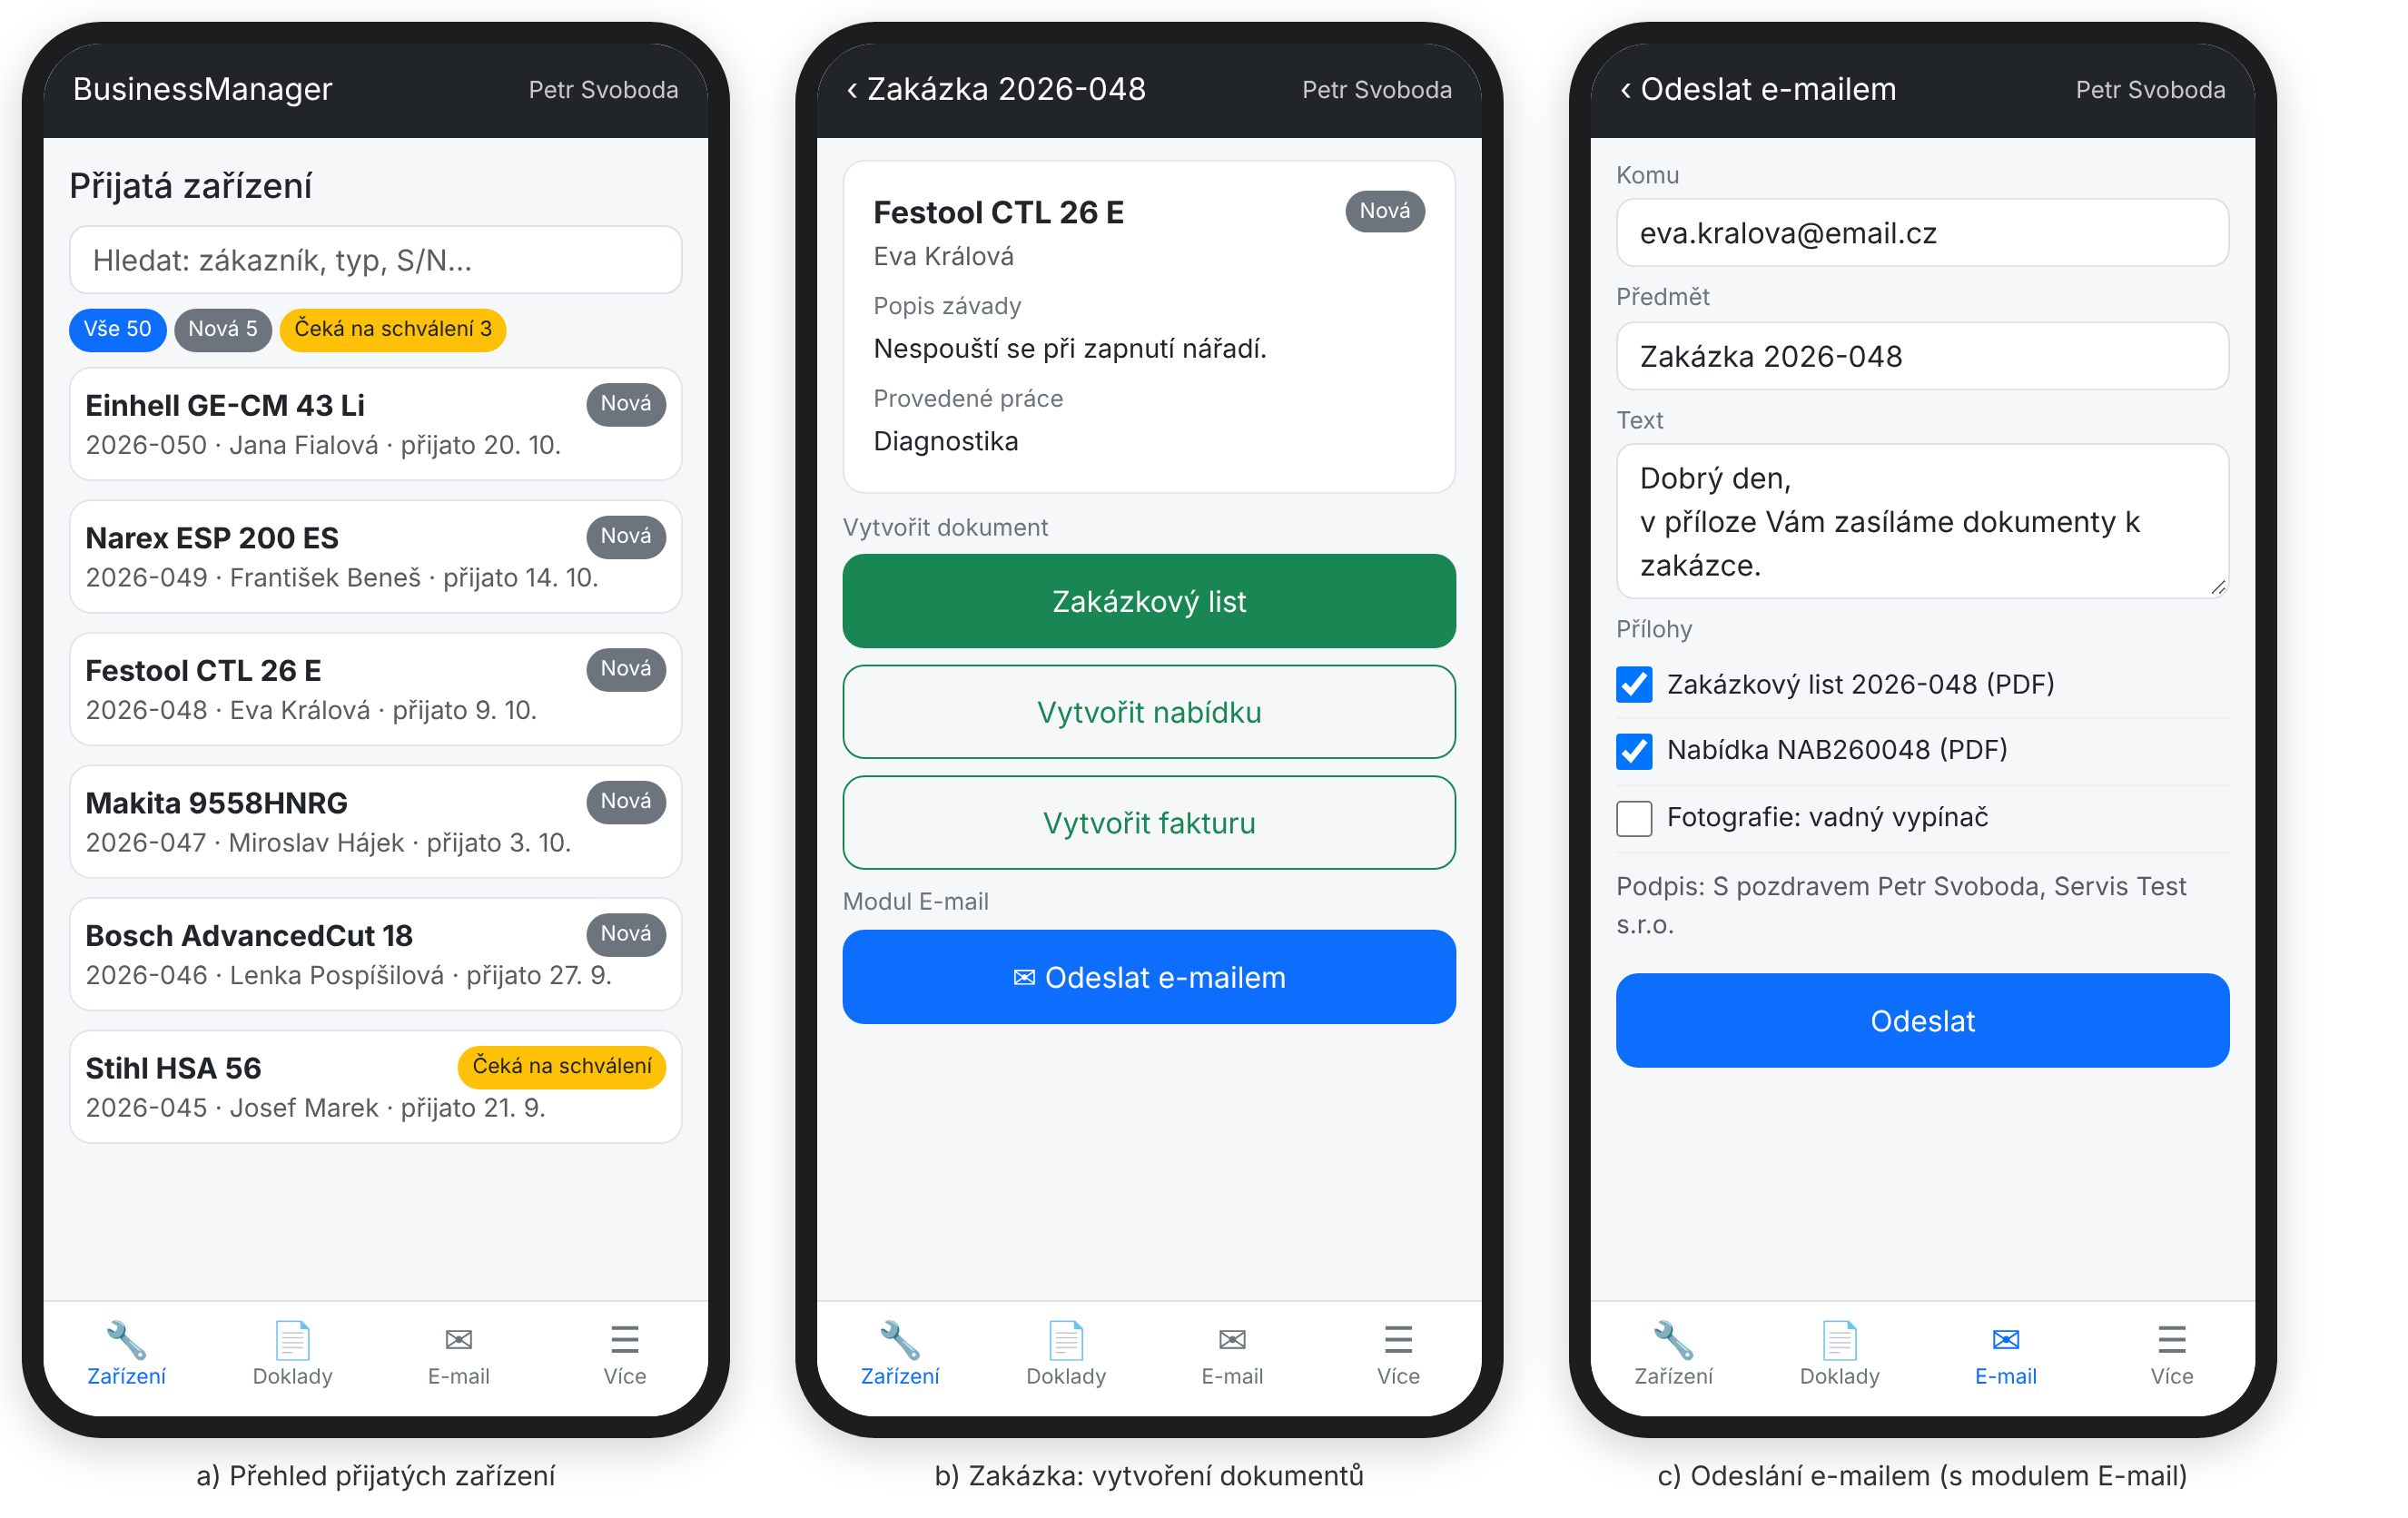
\includegraphics[width=\linewidth]{obrazky/rozvoj/mobilni-navrh.png}
\caption{Návrh zobrazení aplikace na telefonu v~plánovaném modulu Mobilní přístup: a)~přehled přijatých zařízení, b)~vytvoření dokumentů ze zakázky, c)~odeslání e-mailem (zdroj: vlastní návrh, data z~testovací databáze)}\label{obr:mobilni-navrh}
\end{figure}

Mimo moduly zůstávají možností rozvoje úpravy rozhraní podle doporučení z~oddílu~\ref{sec:ui-upravy} a~pohodlnější předávání faktur do účetnictví, pro které aplikace už vytváří elektronickou fakturu ve formátu ISDOC.
